\documentclass[aspectratio=169]{beamer}

\usepackage[utf8]{inputenc}
\usepackage{graphicx}
\usepackage{tikz}
\usetikzlibrary{positioning, arrows.meta, shapes.symbols}
\usepackage{pifont}

\usefonttheme{professionalfonts}

% Theme
\usetheme{Madrid}
\definecolor{ucdgreen}{RGB}{0, 102, 51}
\definecolor{gapred}{RGB}{180, 50, 50}
\definecolor{stepfill}{RGB}{230, 243, 235}
\definecolor{topfill}{RGB}{0, 102, 51}
\definecolor{donefill}{RGB}{200, 230, 210}
\definecolor{nextfill}{RGB}{255, 240, 200}
\usecolortheme[named=ucdgreen]{structure}
\setbeamertemplate{navigation symbols}{}

\title[Research Studies Panel]{Research Studies Panel}
\author[Lainey Ward]{Lainey Ward}
\institute[]{Decarb-AI Centre, School of Civil Engineering\\
Primary supervisor: Dr Fiachra O'Loughlin \\ Co-supervisor: Dr Conor Sweeney}
\date{}

\begin{document}


% --------------------------------------------------
% SLIDE 6: Training & Development — timeline strip
% --------------------------------------------------
\begin{frame}{Training \& Development}

    % --- Credits pill bar ---
    \vspace{0.2em}
    
\begin{tikzpicture}
        \node[font=\footnotesize\bfseries, text=ucdgreen!80!black,
              anchor=west] at (0, 0) {Credits};
        \fill[ucdgreen!35, rounded corners=3pt]
            (1.8, -0.25) rectangle (3.8, 0.25);
        \node[font=\tiny, text=ucdgreen!90!black] at (2.8, 0)
            {ACM41070 (5)};
        \fill[ucdgreen!35, rounded corners=3pt]
            (3.95, -0.25) rectangle (5.95, 0.25);
        \node[font=\tiny, text=ucdgreen!90!black] at (4.95, 0)
            {STAT41130 (5)};
        \fill[nextfill, rounded corners=3pt, draw=orange!40]
            (6.1, -0.25) rectangle (8.1, 0.25);
        \node[font=\tiny, text=orange!80!black] at (7.1, 0)
            {COMP41850 (5)};
        \fill[gray!25, rounded corners=3pt]
            (8.25, -0.25) rectangle (9.75, 0.25);
        \node[font=\tiny, text=gray!70] at (9.0, 0)
            {RPL (15)};
    \end{tikzpicture}

    \vspace{0.3em}

    % --- Training pill bar ---
    
\begin{tikzpicture}
        \node[font=\footnotesize\bfseries, text=ucdgreen!80!black,
              anchor=west] at (0, 0) {Training};
        \fill[ucdgreen!25, rounded corners=3pt]
            (1.8, -0.25) rectangle (4.2, 0.25);
        \node[font=\tiny, text=ucdgreen!90!black] at (3.0, 0)
            {Research integrity};
        \fill[ucdgreen!25, rounded corners=3pt]
            (4.35, -0.25) rectangle (5.95, 0.25);
        \node[font=\tiny, text=ucdgreen!90!black] at (5.15, 0)
            {HPC};
        \fill[ucdgreen!25, rounded corners=3pt]
            (6.1, -0.25) rectangle (8.3, 0.25);
        \node[font=\tiny, text=ucdgreen!90!black] at (7.2, 0)
            {Ark presentation};
        \fill[nextfill, rounded corners=3pt, draw=orange!40]
            (8.45, -0.25) rectangle (10.55, 0.25);
        \node[font=\tiny, text=orange!80!black] at (9.5, 0)
            {DestinE ML};
    \end{tikzpicture}

    \vspace{0.5em}

    % --- Timeline (Apr onwards) ---
    \centering
    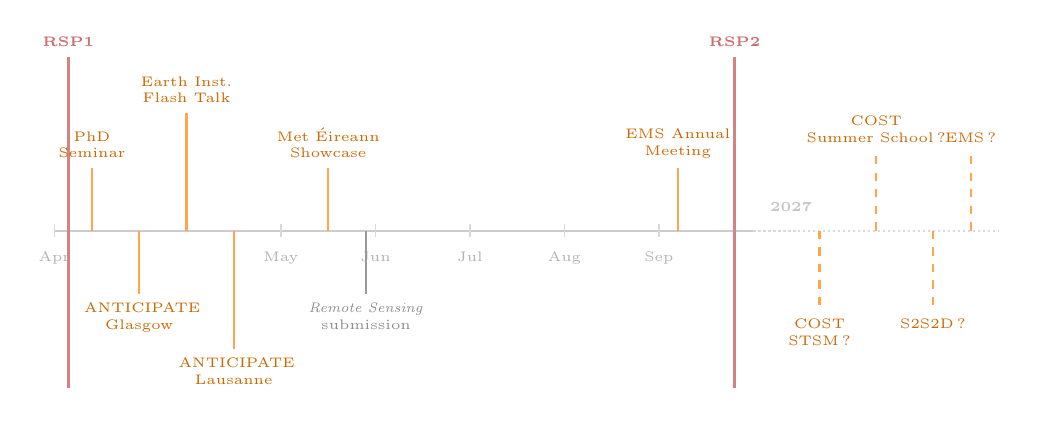
\begin{tikzpicture}[
        xscale=1.2,
        evt/.style={font=\tiny, align=center, text width=2.2cm},
        lbl/.style={font=\tiny, text=gray!60}
    ]

    % Timeline axis — non-uniform spacing to give April more room
    % Apr=0, May=2.4, Jun=3.4, Jul=4.4, Aug=5.4, Sep=6.4
    \draw[thick, gray!40] (0, 0) -- (7.4, 0);

    % Dotted extension for next year
    \draw[thick, gray!30, densely dotted] (7.4, 0) -- (10.0, 0);

    % Month ticks + labels
    \foreach \x/\m in {
        0.0/Apr, 2.4/May, 3.4/Jun, 4.4/Jul, 5.4/Aug, 6.4/Sep}
    {
        \draw[gray!30] (\x, -0.08) -- (\x, 0.08);
        \node[lbl, below=2pt] at (\x, -0.08) {\m};
    }

    % RSP1 marker (7 Apr ~ 0.15)
    \draw[gapred!60, thick] (0.15, -2.0) -- (0.15, 2.2);
    \node[font=\tiny\bfseries, text=gapred!70] at (0.15, 2.4) {RSP1};

    % RSP2 marker (end Sep ~ 7.2)
    \draw[gapred!60, thick] (7.2, -2.0) -- (7.2, 2.2);
    \node[font=\tiny\bfseries, text=gapred!70] at (7.2, 2.4) {RSP2};

    % === APRIL EVENTS (spread across 0–2.4) ===
    % PhD Seminar 9 Apr (above, short)
    \draw[orange!70, thick] (0.4, 0) -- (0.4, 0.8);
    \node[evt, text=orange!80!black, above, text width=1.4cm] at (0.4, 0.8) {PhD\\Seminar};

    % Glasgow 14–15 Apr (below, short)
    \draw[orange!70, thick] (0.9, 0) -- (0.9, -0.8);
    \node[evt, text=orange!80!black, below, text width=1.4cm] at (0.9, -0.8) {ANTICIPATE\\Glasgow};

    % Earth Institute Flash Talk 22 Apr (above, tall — clears PhD Seminar)
    \draw[orange!70, thick] (1.4, 0) -- (1.4, 1.5);
    \node[evt, text=orange!80!black, above, text width=1.4cm] at (1.4, 1.5) {Earth Inst.\\Flash Talk};

    % Lausanne 27–28 Apr (below, tall — clears Glasgow)
    \draw[orange!70, thick] (1.9, 0) -- (1.9, -1.5);
    \node[evt, text=orange!80!black, below, text width=1.4cm] at (1.9, -1.5) {ANTICIPATE\\Lausanne};

    % === MAY–SEP EVENTS ===
    % Met Éireann 20 May (above, short — clear of April cluster)
    \draw[orange!70, thick] (2.9, 0) -- (2.9, 0.8);
    \node[evt, text=orange!80!black, above, text width=1.8cm] at (2.9, 0.8) {Met \'Eireann\\Showcase};

    % Remote Sensing submission end May (below)
    \draw[gray!80, thick] (3.3, 0) -- (3.3, -0.8);
    \node[evt, text=gray!90, below, text width=1.8cm] at (3.3, -0.8) {\textit{Remote Sensing}\\submission};

    % EMS 6–11 Sep (above)
    \draw[orange!70, thick] (6.6, 0) -- (6.6, 0.8);
    \node[evt, text=orange!80!black, above] at (6.6, 0.8) {EMS Annual\\Meeting};

    % === NEXT YEAR 2027 (dotted extension) ===
    \node[font=\tiny\bfseries, text=gray!45] at (7.8, 0.3) {2027};

    \draw[orange!70, thick, dashed] (8.1, 0) -- (8.1, -1.0);
    \node[evt, text=orange!80!black, below, text width=1.8cm] at (8.1, -1.0) {COST\\STSM\,?};

    \draw[orange!70, thick, dashed] (8.7, 0) -- (8.7, 1.0);
    \node[evt, text=orange!80!black, above, text width=1.8cm] at (8.7, 1.0) {COST\\Summer School\,?};

    \draw[orange!70, thick, dashed] (9.3, 0) -- (9.3, -1.0);
    \node[evt, text=orange!80!black, below, text width=1.6cm] at (9.3, -1.0) {S2S2D\,?};

    \draw[orange!70, thick, dashed] (9.7, 0) -- (9.7, 1.0);
    \node[evt, text=orange!80!black, above, text width=1.4cm] at (9.7, 1.0) {EMS\,?};


    \end{tikzpicture}

\end{frame}

% --------------------------------------------------
% BACKUP SLIDE: References
% --------------------------------------------------
\appendix
\begin{frame}{References}

    \scriptsize
    \begin{itemize}\setlength{\itemsep}{0.45em}

    \item Anderson, B.~J., and Coauthors, 2025: What is a drought-to-flood transition? Pitfalls and recommendations for defining consecutive hydrological extreme events. \textit{Hydrol.\ Earth Syst.\ Sci.}, \textbf{29}, 6069--6092.

    \item DeFlorio, M.~J., and Coauthors, 2024: From California's extreme drought to major flooding: Evaluating and synthesizing experimental seasonal and subseasonal forecasts during winter 2022/23. \textit{Bull.\ Amer.\ Meteor.\ Soc.}, \textbf{105}, E84--E104.

    \item Dong, N., H.~Hao, M.~Yang, J.~Wei, S.~Xu, and H.~Kunstmann, 2025: Deep-learning-based sub-seasonal precipitation and streamflow ensemble forecasting over the source region of the Yangtze River. \textit{Hydrol.\ Earth Syst.\ Sci.}, \textbf{29}, 2023--2042.

    \item Kratzert, F., D.~Klotz, C.~Brenner, K.~Schulz, and M.~Herrnegger, 2018: Rainfall--runoff modelling using Long Short-Term Memory (LSTM) networks. \textit{Hydrol.\ Earth Syst.\ Sci.}, \textbf{22}, 6005--6022.

    \item Malik, I., and V.~Mishra, 2025: Sub-seasonal prediction of compound hot and dry extremes in India. \textit{Climate Dyn.}, \textbf{63}, 191.

    \item Mariotti, A., and Coauthors, 2020: Windows of opportunity for skillful forecasts subseasonal to seasonal and beyond. \textit{Bull.\ Amer.\ Meteor.\ Soc.}, \textbf{101}, E608--E625.

    \item Rashid, M.~M., and T.~Wahl, 2022: Hydrologic risk from consecutive dry and wet extremes at the global scale. \textit{Environ.\ Res.\ Commun.}, \textbf{4}, 071001.

    \item Zscheischler, J., and Coauthors, 2020: A typology of compound weather and climate events. \textit{Nat.\ Rev.\ Earth Environ.}, \textbf{1}, 333--347.

    \end{itemize}

\end{frame}

\end{document}